\documentclass[12pt,a4paper]{article}

% Essential packages only
\usepackage{geometry}
\usepackage{hyperref}
\usepackage{booktabs}
\usepackage{array}
\usepackage{xcolor}
\usepackage{listings}
\usepackage{float}
\usepackage{graphicx}
\usepackage{tikz}
\usetikzlibrary{positioning}
\usepackage{tcolorbox}

% Basic document setup
\geometry{margin=1in}
\hypersetup{
    colorlinks=true,
    linkcolor=blue,
    urlcolor=blue
}

% Listings configuration to handle long lines
\lstset{
    basicstyle=\ttfamily\footnotesize,
    breaklines=true,
    breakatwhitespace=true,
    frame=single,
    frameround=tttt,
    captionpos=b,
    numbers=none,
    commentstyle=\itshape\color{gray},
    keywordstyle=\bfseries\color{blue},
    stringstyle=\color{red},
    showstringspaces=false,
    tabsize=4,
    columns=flexible,
    keepspaces=true,
    xleftmargin=0.5cm,
    xrightmargin=0.5cm,
    postbreak=\mbox{\textcolor{red}{$\hookrightarrow$}\space}
}

% Define simple box environments
\newtcolorbox{infobox}{
    colback=blue!5,
    colframe=blue!40!black,
    title=Information
}

\newtcolorbox{technicalbox}{
    colback=gray!5,
    colframe=gray!40!black,
    title=Technical Notes
}

% Simple title setup
\title{CIAF Variables, Interfaces \& Functions Reference}
\author{Denzil James Greenwood}
\date{v1.0.0 - \today}

\begin{document}

% Custom title page
\begin{titlepage}
\begin{center}

\vspace*{1cm}

{\Huge\bfseries CIAF Variables, Interfaces \& Functions Reference}

\vspace{0.5cm}
{\Large\textit{Comprehensive Naming Convention Standards}}

\vspace{1.5cm}

\begin{center}
\begin{infobox}
\centering
\textbf{Authoritative Source of Truth}\\
This document provides comprehensive reference for variable naming conventions, interfaces, and functions used throughout the Cognitive Insight AI Framework (CIAF) codebase. The goal is to ensure consistent naming patterns and provide clarity on variable relationships and cryptographic hierarchies.
\end{infobox}
\end{center}

\vspace{2cm}

{\Large
\textbf{Author:} Denzil James Greenwood\\
\textbf{Version:} 1.0.0\\
\textbf{Date:} October 23, 2025\\
\textbf{Document Type:} Technical Reference
}

\vspace{2cm}

\begin{center}
\begin{technicalbox}
\textbf{Usage Guidelines}
\begin{itemize}
\item This document serves as the single source of truth for CIAF naming conventions
\item All code implementations must conform to patterns specified herein
\item Consult this reference when adding new variables or refactoring existing code
\item Maintain cryptographic hierarchy relationships as documented
\end{itemize}
\end{technicalbox}
\end{center}

\vfill

{\small
\textbf{Classification:} Technical Documentation\\
\textbf{Distribution:} Internal Development Team\\
\textbf{Last Updated:} \today
}

\end{center}
\end{titlepage}

% Abstract
\begin{abstract}
The Cognitive Insight AI Framework (CIAF) Variables Reference provides comprehensive documentation for naming conventions, interface patterns, and function signatures used throughout the CIAF codebase. This document establishes consistent naming standards for cryptographic variables, anchor hierarchies, receipt management, and API interfaces. It serves as the authoritative source for developers implementing CIAF components, ensuring code clarity, maintainability, and adherence to cryptographic security principles. The reference covers core naming patterns, suffix conventions, variable relationships, and best practices for maintaining consistency across the framework's distributed architecture.
\end{abstract}

\newpage
\tableofcontents
\newpage

\section{Document Purpose and Scope}

This document provides a comprehensive reference for variable naming conventions, interfaces, and functions used throughout the Cognitive Insight AI Framework (CIAF) codebase. The primary objectives are:

\begin{itemize}
\item \textbf{Consistency Enforcement:} Establish uniform naming patterns across all CIAF components
\item \textbf{Clarity Provision:} Distinguish between related but distinct variable types (e.g., \texttt{modelAnchor} vs \texttt{modelAnchorRef})
\item \textbf{Hierarchy Documentation:} Define cryptographic relationships and derivation chains
\item \textbf{Interface Standardization:} Specify function signatures and protocol implementations
\end{itemize}

\subsection{Document Authority}

This document serves as the \textbf{single source of truth} for CIAF naming conventions. All code implementations, documentation, and technical specifications must conform to the patterns and standards defined herein.

\subsection{Version Control}

\begin{tabular}{@{}lll@{}}
\toprule
Version & Date & Changes \\
\midrule
1.0.0 & October 23, 2025 & Initial comprehensive reference \\
\bottomrule
\end{tabular}

\section{Naming Convention Principles}

\subsection{Core Naming Patterns}

The CIAF framework employs a hierarchical naming system based on the following conventions:

\begin{description}
\item[\textbf{snake\_case}] Primary convention for variables, functions, and module names
\item[\textbf{PascalCase}] Used for classes, enums, and dataclasses
\item[\textbf{UPPER\_CASE}] Used for constants and enum values
\item[\textbf{Descriptive suffixes}] Added to indicate variable purpose or type
\end{description}

\subsection{Suffix Conventions}

The framework uses standardized suffixes to indicate variable purpose and cryptographic properties:

\begin{table}[H]
\centering
\caption{Standard Suffix Conventions}
\begin{tabular}{@{}ll@{}}
\toprule
\textbf{Suffix} & \textbf{Purpose} \\
\midrule
\texttt{\_anchor} & Cryptographic anchor objects/bytes (internal form) \\
\texttt{\_anchor\_hex} & Hex-encoded anchor strings (external/AAD form) \\
\texttt{\_anchor\_ref} & Opaque reference/ID strings pointing to anchors \\
\texttt{\_ref} & References or IDs pointing to anchors/objects \\
\texttt{\_hash} & SHA-256 or other cryptographic hash values \\
\texttt{\_digest} & Content-derived cryptographic digests \\
\texttt{\_root} & Merkle tree root hashes \\
\texttt{\_id} & Unique identifiers (usually strings) \\
\texttt{\_hex} & Hex-encoded byte values \\
\texttt{\_bytes} & Raw byte data \\
\texttt{\_pem} & PEM-encoded cryptographic keys \\
\texttt{\_metadata} & Structured metadata objects \\
\bottomrule
\end{tabular}
\end{table}

\section{Core Cryptographic Variables}

\subsection{Anchor-Related Variables}

The CIAF framework implements a hierarchical anchor system for cryptographic integrity. The following variables represent different aspects of this system:

\begin{lstlisting}[caption=Master Anchors]
# Master anchors (top-level derivation)
master_anchor: bytes                    # Root anchor derived from password + salt
master_password: str                    # Password for master anchor derivation

# Hierarchical anchors
dataset_anchor: bytes                   # Derived from master_anchor + dataset_hash
model_anchor: bytes                     # Derived from master_anchor + model_hash
capsule_anchor: bytes                   # Derived from dataset_anchor + capsule_id
\end{lstlisting}

\begin{lstlisting}[caption=Anchor Hex Representations]
# Anchor hex representations
dataset_anchor_hex: str                 # Hex-encoded dataset anchor
model_anchor_hex: str                   # Hex-encoded model anchor
capsule_anchor_hex: str                 # Hex-encoded capsule anchor
\end{lstlisting}

\begin{lstlisting}[caption=Anchor References and IDs]
# Anchor references/IDs
anchor_id: str                          # Unique identifier for anchor
anchor_ref: str                         # Reference to existing anchor
\end{lstlisting}

\subsection{Hash Variables}

Cryptographic hash variables follow standardized naming patterns to indicate their purpose and derivation:

\begin{lstlisting}[caption=Content Hashes]
# Content hashes
dataset_hash: str                       # SHA-256 hash of dataset content
model_hash: str                         # SHA-256 hash of model parameters
content_hash: str                       # Generic content hash
schema_digest: str                      # Hash of data schema
params_root: str                        # Merkle root of model parameters
arch_root: str                          # Merkle root of model architecture
\end{lstlisting}

\begin{lstlisting}[caption=Cryptographic Digests]
# Cryptographic digests
leaf_hash: str                          # Individual Merkle tree leaf
merkle_root: str                        # Merkle tree root hash
root_hash: str                          # Generic root hash
split_assignment_digest: str            # Hash of train/val/test split assignments
hp_digest: str                          # Hyperparameter configuration digest
env_digest: str                         # Training environment digest
\end{lstlisting}

\subsection{Signature Variables}

Digital signature variables maintain clear distinctions between different representations and key types:

\begin{lstlisting}[caption=Digital Signatures]
# Digital signatures
signature: str                          # Base64-encoded Ed25519 signature
signature_bytes: bytes                  # Raw signature bytes
merkle_signature: str                   # Signature over Merkle root
\end{lstlisting}

\begin{lstlisting}[caption=Keys and Key Management]
# Keys and key management
private_key: Ed25519PrivateKey         # Ed25519 private key object
public_key: Ed25519PublicKey           # Ed25519 public key object
key_id: str                            # Unique key identifier
public_key_pem: str                    # PEM-encoded public key
private_key_pem: str                   # PEM-encoded private key
key_fingerprint: str                   # SHA-256 fingerprint of public key
\end{lstlisting}

\section{LCM (Lazy Capsule Materialization) Variables}

\subsection{Core LCM Objects}

The Lazy Capsule Materialization system uses specialized dataclasses and managers for different aspects of the AI lifecycle:

\begin{lstlisting}[caption=Anchor Objects (Dataclasses)]
# Anchor objects (dataclasses)
dataset_anchor: LCMDatasetAnchor       # Dataset anchor with metadata
model_anchor: LCMModelAnchor           # Model anchor with metadata
training_anchor: LCMTrainingAnchor     # Training session anchor
deployment_anchor: LCMDeploymentAnchor # Deployment anchor
\end{lstlisting}

\begin{lstlisting}[caption=Manager Objects]
# Manager objects
dataset_manager: LCMDatasetManager     # Dataset management
model_manager: LCMModelManager         # Model management  
training_manager: LCMTrainingManager   # Training session management
deployment_manager: LCMDeploymentManager # Deployment management
\end{lstlisting}

\subsection{Receipt Variables}

Receipt variables represent different levels of audit detail and materialization:

\begin{lstlisting}[caption=Receipt Objects]
# Receipt objects
lightweight_receipt: LightweightReceipt    # Minimal audit receipt
inference_receipt: InferenceReceipt        # Full inference audit record
training_receipt: TrainingReceipt          # Training session receipt
\end{lstlisting}

\begin{lstlisting}[caption=Receipt Fields]
# Receipt fields
receipt_id: str                            # Unique receipt identifier
inference_id: str                          # Unique inference identifier
capsule_id: str                            # Capsule identifier
session_id: str                            # Training/inference session ID
committed_at: str                          # Receipt creation timestamp (RFC 3339 Z)
\end{lstlisting}

\subsection{Split and Dataset Variables}

Dataset management variables handle data organization and metadata:

\begin{lstlisting}[caption=Dataset Splits]
# Dataset splits
train_split: DatasetSplit              # Training data split
val_split: DatasetSplit                # Validation data split  
test_split: DatasetSplit               # Test data split
split_assignment: Dict[str, str]       # Record ID to split mapping
\end{lstlisting}

\begin{lstlisting}[caption=Dataset Metadata]
# Dataset metadata
dataset_metadata: DatasetMetadata      # Comprehensive dataset info
split_metadata: SplitMetadata          # Split-specific metadata
schema_metadata: Dict[str, Any]        # Data schema information
\end{lstlisting}

\section{API and Interface Variables}

\subsection{Protocol Interface Variables}

The CIAF framework uses protocol-based interfaces for core cryptographic and storage operations:

\begin{lstlisting}[caption=Core Protocol Implementations]
# Core protocol implementations
signer: Signer                         # Digital signature protocol
rng: RNG                              # Random number generator protocol
merkle: Merkle                        # Merkle tree protocol
anchor_deriver: AnchorDeriver         # Anchor derivation protocol
anchor_store: AnchorStore             # Anchor storage protocol
\end{lstlisting}

\begin{lstlisting}[caption=API Handler Protocols]
# API handler protocols
dataset_api_handler: DatasetAPIHandler # Dataset API operations
model_api_handler: ModelAPIHandler     # Model API operations
audit_api_handler: AuditAPIHandler     # Audit API operations
\end{lstlisting}

\subsection{Framework Objects}

Governance framework variables provide domain-specific compliance implementations:

\begin{lstlisting}[caption=Governance Frameworks]
# Governance frameworks
governance_framework: AIGovernanceFramework    # Base governance
banking_framework: BankingAIGovernanceFramework # Banking-specific
healthcare_framework: HealthcareAIGovernanceFramework # Healthcare-specific
government_framework: GovernmentAIGovernanceFramework # Government-specific
\end{lstlisting}

\begin{lstlisting}[caption=Organization and Configuration]
# Organization and config
organization_id: str                   # Unique organization identifier
framework_version: str                 # Framework version string
governance_config: Dict[str, Any]      # Configuration parameters
compliance_history: List[Dict]         # Historical compliance events
\end{lstlisting}

\section{Enum and Constant Variables}

\subsection{Core Enums}

Enumeration variables provide type safety and standardized values:

\begin{lstlisting}[caption=Core Enums]
# Record types
record_type: RecordType               # DATASET, MODEL, INFERENCE, ANCHOR, etc.

# Algorithms
hash_algorithm: HashAlgorithm         # SHA256, SHA3_256, BLAKE3
signature_algorithm: SignatureAlgorithm # ED25519, MOCK

# Consent management
consent_status: ConsentStatus         # GRANTED, DENIED, EXPIRED, etc.
consent_type: ConsentType             # EXPLICIT, IMPLIED, PARENTAL, etc.
consent_scope: ConsentScope           # DATA_PROCESSING, SHARING, etc.
\end{lstlisting}

\subsection{Constant Variables}

Framework constants ensure consistency across implementations:

\begin{lstlisting}[caption=Cryptographic Constants]
# Cryptographic constants
SALT_LENGTH: int = 16                  # Salt length in bytes
PBKDF2_ITERATIONS: int = 100_000      # PBKDF2 iteration count
KDF_DKLEN: int = 32                   # Key derivation output length
HASH_OUTPUT_LENGTH: int = 64          # SHA-256 hex output length

# Default algorithms
DEFAULT_HASH_FUNCTION: str = "sha256"
DEFAULT_SIGNATURE_ALGORITHM: str = "ed25519"
DEFAULT_PUBKEY_ID: str = "ciaf_production_key_001"

# Schema versions
ANCHOR_SCHEMA_VERSION: str = "1.0"
MERKLE_POLICY_VERSION: str = "1.0"

# Prefixes
EVENT_ID_PREFIX: str = "evt"
\end{lstlisting}

\section{Function Naming Patterns}

\subsection{Cryptographic Functions}

Function naming follows consistent patterns that reflect their cryptographic purpose:

\begin{lstlisting}[caption=Hash Functions]
# Hash functions
def sha256_hash(data: bytes) -> str
def blake3_hash(data: bytes) -> str  
def sha3_256_hash(data: bytes) -> str
def compute_hash(data: bytes, algorithm: str) -> str
def hmac_sha256(key: bytes, data: bytes) -> str
\end{lstlisting}

\begin{lstlisting}[caption=Anchor Derivation Functions]
# Anchor derivation functions
def derive_master_anchor(password: str, salt: bytes) -> bytes
def derive_dataset_anchor(master_anchor: bytes, dataset_hash: str) -> bytes
def derive_model_anchor(master_anchor: bytes, model_hash: str) -> bytes
def derive_capsule_anchor(dataset_anchor: bytes, capsule_id: str) -> bytes
\end{lstlisting}

\begin{lstlisting}[caption=Encryption Functions]
# Encryption functions
def encrypt_aes_gcm(key: bytes, plaintext: bytes, aad: bytes) -> tuple
def decrypt_aes_gcm(key: bytes, ciphertext: bytes, nonce: bytes, 
                   tag: bytes, aad: bytes) -> bytes
def make_aad(dataset_anchor_hex: str, capsule_id: str, 
            policy_id: str) -> bytes
\end{lstlisting}

\subsection{LCM Management Functions}

LCM management functions follow consistent creation and manipulation patterns:

\begin{lstlisting}[caption=Manager Creation Functions]
# Manager creation functions
def create_dataset_manager(policy: LCMPolicy, rng: RNG) -> LCMDatasetManager
def create_model_manager(policy: LCMPolicy, rng: RNG) -> LCMModelManager
def create_training_manager(model_anchor: LCMModelAnchor, 
                          datasets: List) -> LCMTrainingManager
\end{lstlisting}

\begin{lstlisting}[caption=Receipt Generation Functions]
# Receipt generation functions
def generate_lightweight_receipt(inference_data: Dict) -> LightweightReceipt
def materialize_full_receipt(lightweight_receipt: LightweightReceipt) -> InferenceReceipt
\end{lstlisting}

\begin{lstlisting}[caption=Validation Functions]
# Validation functions
def validate_anchor_chain(anchor_chain: List[str]) -> bool
def verify_merkle_proof(leaf_hash: str, proof: List, root: str) -> bool
def validate_governance_requirements(system_id: str, 
                                   requirements: Dict) -> Dict
\end{lstlisting}

\subsection{API Functions}

API functions implement standard CRUD patterns with consistent naming:

\begin{lstlisting}[caption=CRUD Operations]
# CRUD operations
def create_dataset(dataset_id: str, metadata: Dict) -> Dict
def get_dataset(dataset_id: str) -> Optional[Dict]
def update_dataset(dataset_id: str, updates: Dict) -> Dict
def delete_dataset(dataset_id: str) -> bool
\end{lstlisting}

\begin{lstlisting}[caption=Assessment Functions]
# Assessment functions
def assess_compliance(system_id: str, assessment_type: str) -> Dict
def generate_audit_report(system_id: str, report_type: str) -> Dict
def record_governance_event(event_type: str, event_data: Dict) -> str
\end{lstlisting}

\section{Variable Relationship Patterns}

\subsection{Anchor Relationships}

The cryptographic anchor system maintains clear hierarchical relationships:

\begin{lstlisting}[caption=Anchor Hierarchy]
# Base anchor and its references
model_anchor: LCMModelAnchor           # Full anchor object with metadata
model_anchor_ref: str                  # Reference ID to the anchor
model_anchor_hex: str                  # Hex representation for AAD/binding
model_hash: str                        # Content hash used to derive anchor

# Chain relationships
master_anchor: bytes                   # Root of derivation chain
dataset_anchor: bytes                  # Derived from master_anchor + dataset_hash
capsule_anchor: bytes                  # Derived from dataset_anchor + capsule_id
\end{lstlisting}

\subsection{Receipt Relationships}

Receipt variables represent different stages of audit trail materialization:

\begin{lstlisting}[caption=Receipt Progression]
# Receipt progression
lightweight_receipt: LightweightReceipt    # Minimal storage during operation
inference_receipt: InferenceReceipt        # Materialized full audit record
receipt_id: str                            # Unique identifier linking them
receipt_ref: str                           # Reference used in other contexts
\end{lstlisting}

\subsection{Merkle Tree Relationships}

Merkle tree variables maintain cryptographic proof relationships:

\begin{lstlisting}[caption=Merkle Tree Structure]
# Tree construction
leaf_hash: str                         # Individual operation hash
merkle_path: List[Tuple[str, str]]     # Proof path from leaf to root
merkle_root: str                       # Root hash of the tree
merkle_signature: str                  # Digital signature over root
\end{lstlisting}

\section{Best Practices}

\subsection{Consistent Suffixing}

\begin{itemize}
\item Always use \texttt{\_anchor} for anchor objects/bytes
\item Use \texttt{\_ref} or \texttt{\_id} for string references to anchors
\item Use \texttt{\_hex} when converting bytes to hex strings
\item Use \texttt{\_hash} for content-derived cryptographic hashes
\end{itemize}

\subsection{Type Clarity}

\begin{itemize}
\item Include type hints for all function parameters and returns
\item Use descriptive variable names that indicate their purpose
\item Distinguish between raw bytes, hex strings, and object references
\end{itemize}

\subsection{Hierarchical Naming}

\begin{itemize}
\item Reflect the cryptographic hierarchy in variable names
\item Use consistent prefixes for related operations (e.g., \texttt{derive\_*\_anchor})
\item Group related variables with common prefixes
\end{itemize}

\subsection{Documentation}

\begin{itemize}
\item Include docstrings explaining the relationship between variables
\item Document the cryptographic properties of anchor variables
\item Explain when to use different forms of the same conceptual data
\end{itemize}

\section{Variable Cross-Reference Index}

\subsection{Primary Anchor Variables}

The CIAF anchor hierarchy consists of two types of relationships:

\paragraph{Cryptographic Derivations} use HMAC-SHA256 for secure hierarchical key derivation:
\begin{itemize}
\item \texttt{master\_anchor} ← derived from password + salt via PBKDF2
\item \texttt{dataset\_anchor} ← derived from \texttt{master\_anchor} + dataset\_hash
\item \texttt{model\_anchor} ← derived from \texttt{master\_anchor} + model\_hash  
\item \texttt{capsule\_anchor} ← derived from \texttt{dataset\_anchor} + capsule\_id
\end{itemize}

\paragraph{Composite Objects} reference anchors but compute their own hashes:
\begin{itemize}
\item \texttt{training\_session} ← Merkle root of [model\_anchor, datasets\_root, \linebreak training\_snapshot]
\item \texttt{deployment\_anchor} ← Hash of deployment metadata + infrastructure config
\end{itemize}

\begin{center}
\resizebox{0.95\textwidth}{!}{
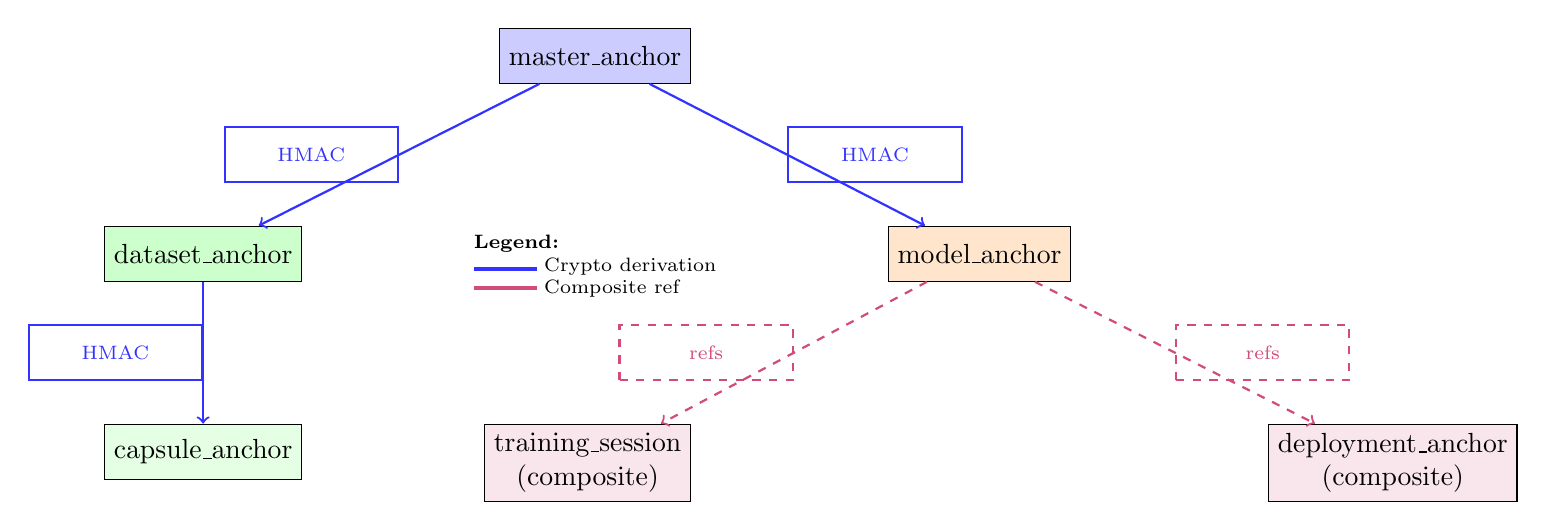
\begin{tikzpicture}[
    node distance=1.8cm and 2.5cm,
    every node/.style={rectangle, draw, align=center, minimum width=2.2cm, minimum height=0.7cm},
    crypto/.style={->, thick, blue!80},
    composite/.style={->, thick, purple!70, dashed},
    object/.style={rectangle, draw, align=center, minimum width=2.2cm, minimum height=0.7cm, fill=purple!10}
]

% Master anchor at the top
\node (master) [fill=blue!20] {master\_anchor};

% Second level: dataset and model anchors (direct crypto derivations)
\node (dataset) [below left=of master, fill=green!20] {dataset\_anchor};
\node (model) [below right=of master, fill=orange!20] {model\_anchor};

% Third level: capsule anchor (crypto derivation from dataset)
\node (capsule) [below=of dataset, fill=green!10] {capsule\_anchor};

% LCM composite objects (not direct crypto derivations)
\node (training) [below left=of model, object] {training\_session\\(composite)};
\node (deployment) [below right=of model, object] {deployment\_anchor\\(composite)};

% Cryptographic derivation arrows (solid blue)
\draw [crypto] (master) -- (dataset) node[midway, left, font=\scriptsize] {HMAC};
\draw [crypto] (master) -- (model) node[midway, right, font=\scriptsize] {HMAC};
\draw [crypto] (dataset) -- (capsule) node[midway, left, font=\scriptsize] {HMAC};

% Composite relationship arrows (dashed purple)
\draw [composite] (model) -- (training) node[midway, left, font=\scriptsize] {refs};
\draw [composite] (model) -- (deployment) node[midway, right, font=\scriptsize] {refs};

% Legend
\node [below=1.8cm of master, draw=none, align=left, font=\scriptsize] {
  \textbf{Legend:}\\
  \textcolor{blue!80}{\rule{0.8cm}{1.5pt}} Crypto derivation\\
  \textcolor{purple!70}{\rule[0.4ex]{0.8cm}{1.5pt}} Composite ref
};

\end{tikzpicture}
}
\end{center}

\subsection{Hash Chain Variables}

The following variables are used in cryptographic derivation functions:

\begin{itemize}
\item \texttt{dataset\_hash} → used in \texttt{derive\_dataset\_anchor(master\_anchor,} \\
\texttt{dataset\_hash)}
\item \texttt{model\_hash} → used in \texttt{derive\_model\_anchor(master\_anchor, model\_hash)}
\item \texttt{capsule\_id} → used in \texttt{derive\_capsule\_anchor(dataset\_anchor, capsule\_id)}
\item \texttt{params\_root} → Merkle root of model parameters
\item \texttt{arch\_root} → Merkle root of architecture specification
\item \texttt{hp\_digest} → Hash of hyperparameters
\item \texttt{env\_digest} → Hash of training environment
\end{itemize}

\paragraph{Implementation Note:} All cryptographic derivations use HMAC-SHA256 with the parent anchor as the key and the child identifier as the data. This ensures cryptographic binding and prevents anchor forgery.

\subsection{Receipt Chain Variables}

\begin{itemize}
\item \texttt{lightweight\_receipt} → minimal audit record
\item \texttt{inference\_receipt} → full materialized record
\item \texttt{training\_receipt} → training session record
\item Connected by \texttt{receipt\_id} and \texttt{inference\_id}
\end{itemize}

\subsection{API Object Variables}

\begin{itemize}
\item \texttt{*\_manager} objects handle lifecycle operations
\item \texttt{*\_api\_handler} objects handle HTTP/API operations  
\item \texttt{governance\_framework} objects handle compliance
\item Connected through dependency injection patterns
\end{itemize}

\section{Implementation Guidelines}

\subsection{New Variable Introduction}

When introducing new variables to the CIAF codebase:

\begin{enumerate}
\item Consult this reference for appropriate naming patterns
\item Ensure suffix conventions align with variable purpose
\item Document cryptographic relationships in code comments
\item Update this reference document when new patterns are established
\end{enumerate}

\subsection{Code Review Checklist}

During code reviews, verify:

\begin{itemize}
\item Variable names follow established suffix conventions
\item Type hints are present and accurate
\item Cryptographic hierarchy relationships are preserved
\item Function naming patterns align with documented standards
\end{itemize}

\subsection{Refactoring Guidelines}

When refactoring existing code:

\begin{itemize}
\item Maintain backward compatibility where possible
\item Update variable names to conform to current standards
\item Preserve cryptographic security properties
\item Update documentation to reflect changes
\end{itemize}

\newpage

\section*{Conclusion}

This Variables Reference serves as the comprehensive authority for CIAF naming conventions, ensuring consistency, clarity, and maintainability across the framework's distributed architecture. By adhering to these standards, developers can create code that is both cryptographically secure and easily understood by team members.

The hierarchical naming system reflects the underlying cryptographic relationships, making code review and security analysis more effective. Regular consultation of this reference during development and code review processes will maintain the high standards required for production AI governance systems.

\section*{Author Information}

\textbf{Denzil James Greenwood} is the creator of the Cognitive Insight AI Framework and inventor of the Lazy Capsule Materialization process. This Variables Reference represents the canonical standards for CIAF development and serves as the authoritative guide for naming conventions across all framework components.

\textbf{Institutional Affiliation:} Independent Researcher \\
\textbf{Contact:} founder@cognitiveinsight.ai \\
\textbf{ORCID:} [To be assigned]

\section*{Copyright Notice}

\begin{infobox}
\textbf{Legal Notice}\\
© 2025 Denzil James Greenwood \\
This Variables Reference, \textit{``CIAF Variables, Interfaces \& Functions Reference,''} \\
is licensed under the \href{https://creativecommons.org/licenses/by/4.0/}{Creative Commons Attribution 4.0 International License (CC BY 4.0)}.

All accompanying source code is released under the \href{https://www.apache.org/licenses/LICENSE-2.0}{Apache License 2.0}. \\
Cognitive Insight\texttrademark{} and Lazy Capsule Materialization (LCM)\texttrademark{} are trademarks of Denzil James Greenwood.
\end{infobox}

\end{document}